
%(BEGIN_QUESTION)
% Copyright 2015, Tony R. Kuphaldt, released under the Creative Commons Attribution License (v 1.0)
% This means you may do almost anything with this work of mine, so long as you give me proper credit

\noindent

\vskip 5pt






\vskip 5pt
\begin{center}
\textbf{HMI -- Nivå 2 }
\vskip 5pt 
\textbf{Arbidsoppdrag på Stasjon 3/4}
\vskip 5pt 
\textbf{Lage HMI til reguleringsstasjon}
\end{center}

\vskip 10pt 
\textbf{Introdusjon}
Denne oppgaven bygger på programmet du har laget i oppgaven programmering av reguleringsstasjon. De anbefales å gjøre disse oppgavene sammen. 



\vskip 5pt 
Du skal lage Følgende HMI bilder.
\begin{itemize}[noitemsep]
\item Level2 For daglig betjening av stasjonen
\item Level3 Som gir en P\&ID oversikt over stasjonen
\item Level4 for optimalisering av nivåregulering
\item Level4 for optimalisering av strømnings regulering
\end{itemize}

 
\vskip 5pt 

%$$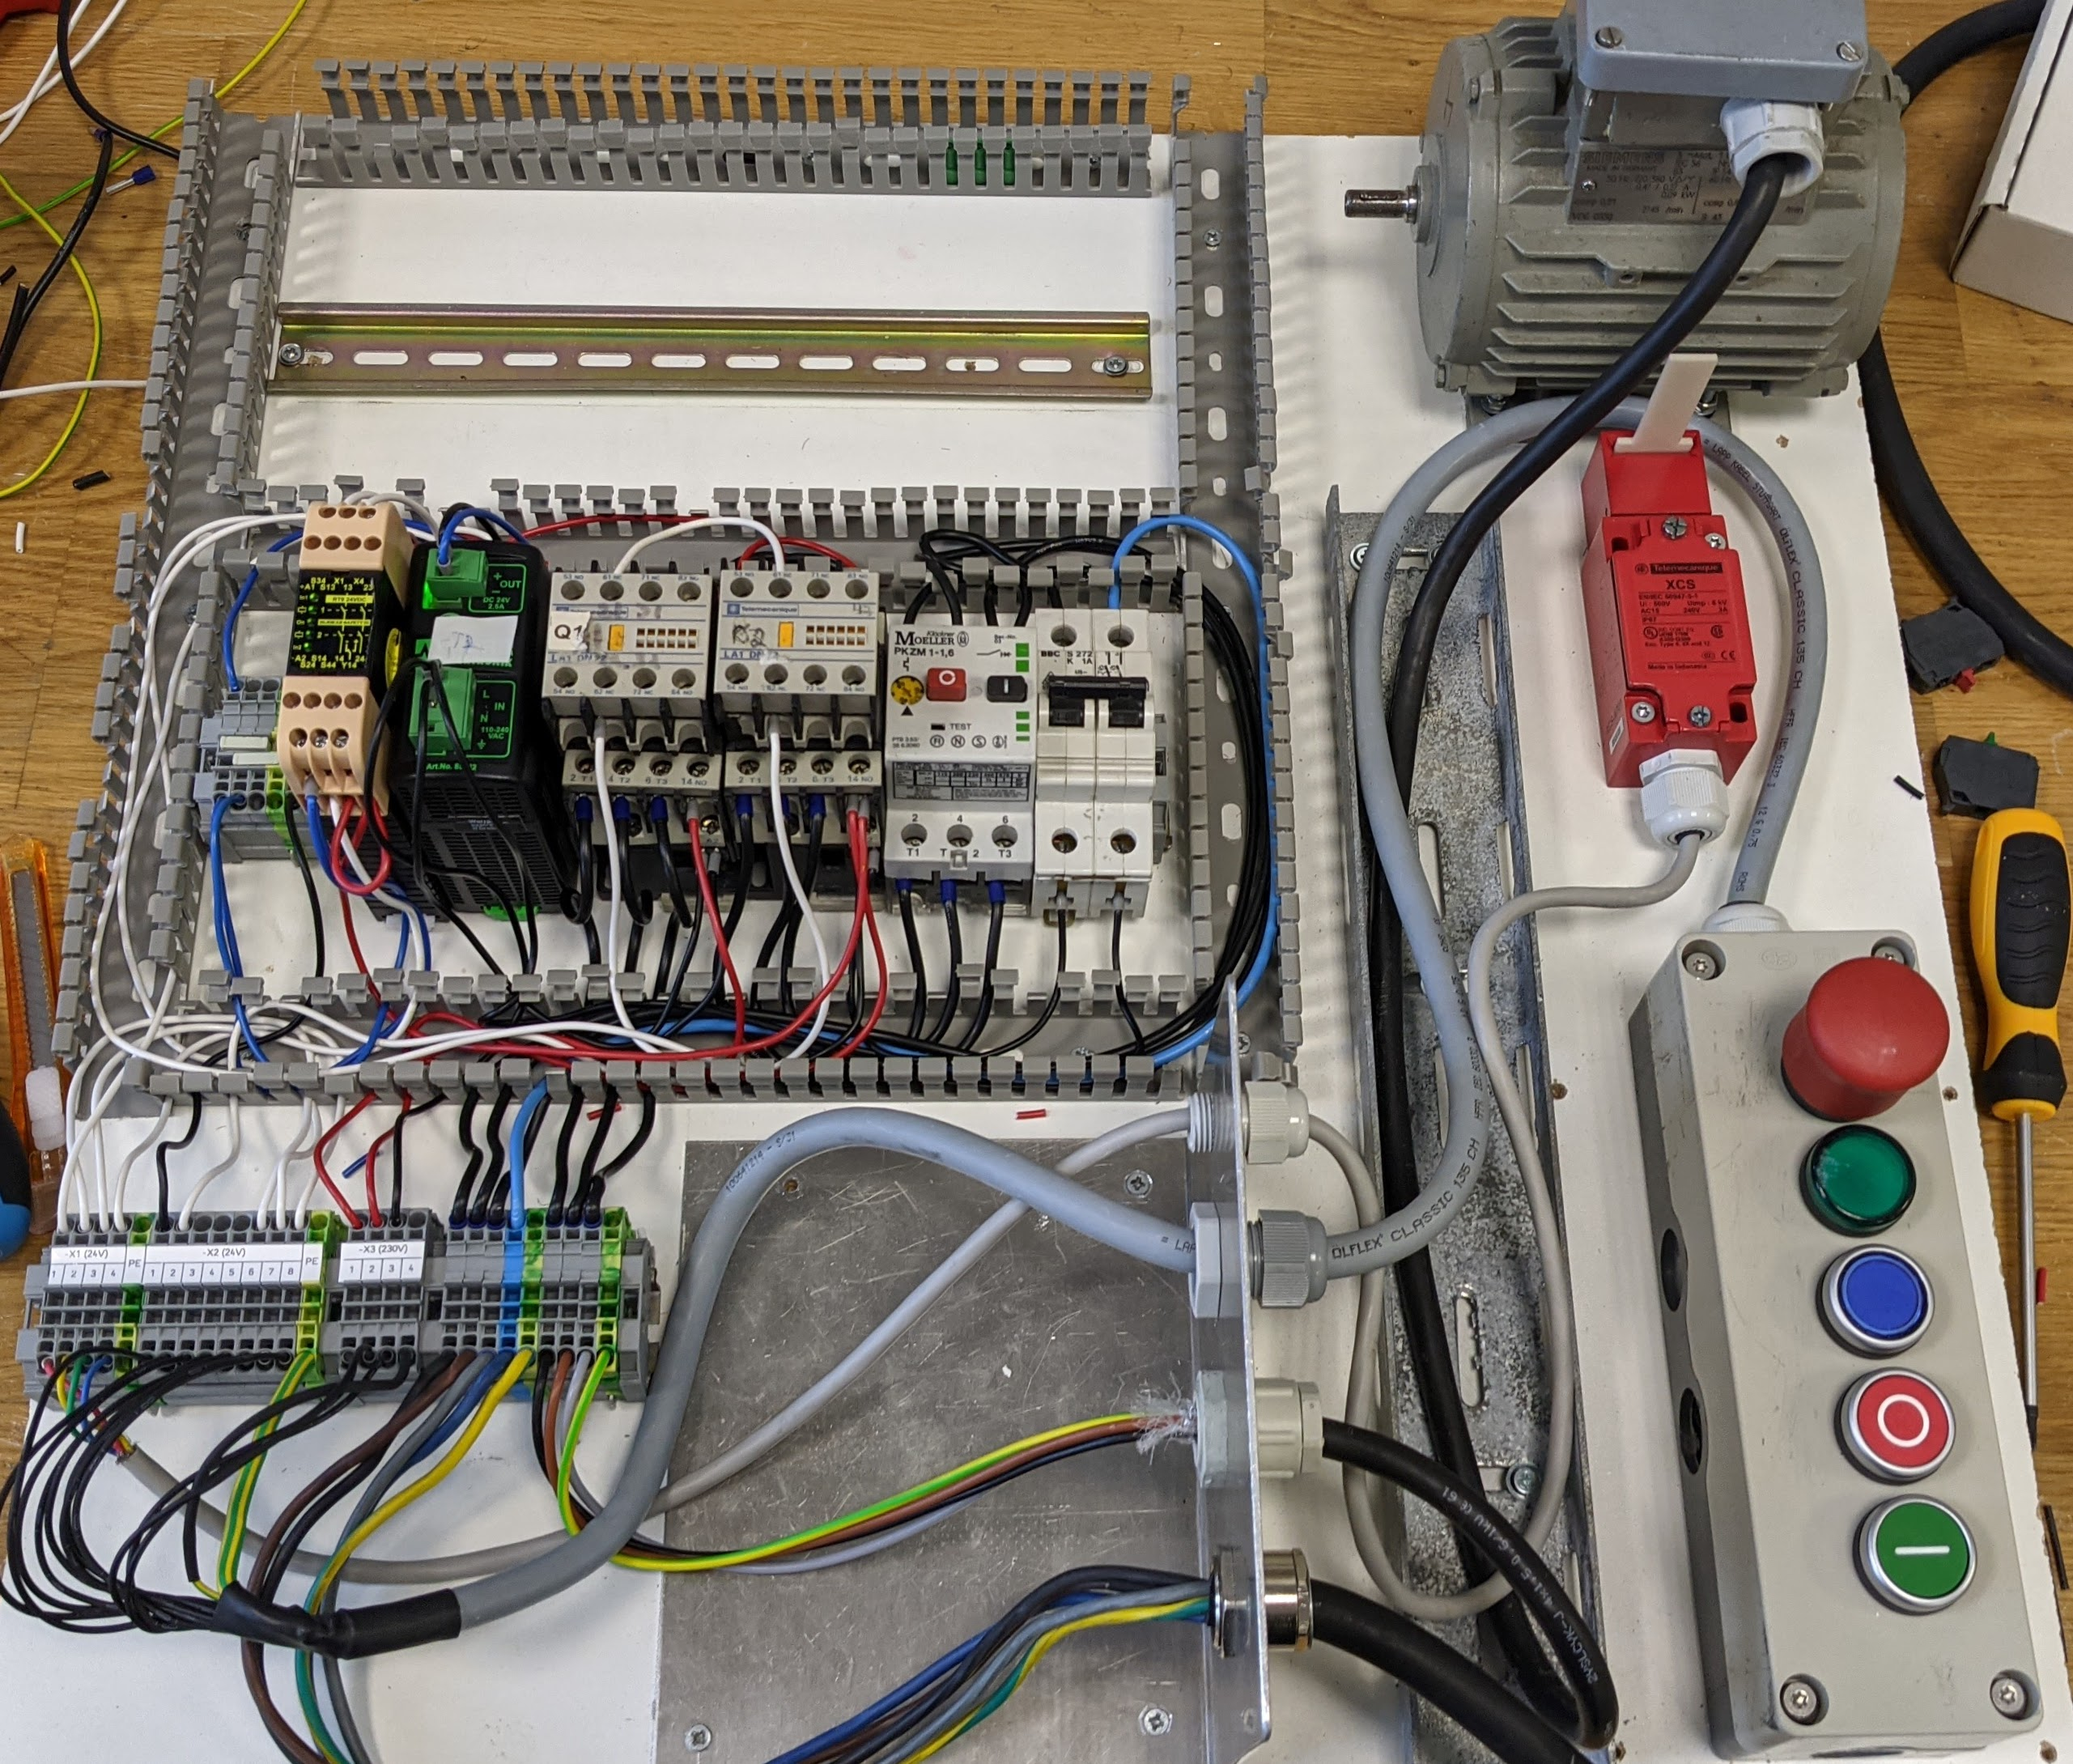
\includegraphics[width=13cm]{i04821x01.jpg}$$\\

\vskip 10pt 
\textbf{Teorioppgaver}

\vskip 5pt 

\vskip 10pt 
\textbf{Planlegging}


\vskip 10pt 
\textbf{Gjennomføring}

\vskip 10pt 
\textbf{Dokumentasjon}

Beskriv hvordan du planlegger, gjennomfører og dokumenterer denne jobben. 


















\underbar{file i04830}
\vfil \eject
%(END_QUESTION)





%(BEGIN_ANSWER)


%(END_ANSWER)





%(BEGIN_NOTES)


%INDEX% Arbeisdoppdrag, HMI, Nivå 2, Stasjon03/04, Lage HMI til reguleringsstasjon. 

%(END_NOTES)


